\documentclass{article}

\usepackage{graphicx}
\usepackage{mathtools}
\usepackage{amsfonts}
\usepackage{amssymb}
\usepackage{amsmath}
\usepackage{tikz}
\usepackage{forest}
\usepackage{xcolor}
\usepackage{bussproofs}
\EnableBpAbbreviations
\usepackage{geometry}
\usepackage{minted}
\usepackage{csquotes}

\usetikzlibrary{arrows,shapes,automata,petri,positioning,calc,fit}
\tikzset{
    fsa-point/.style={
        circle,
        draw=black,
        minimum size=3pt
    },
    asg-point/.style={
        circle,
        draw=black,
        minimum size=3pt
    },
    every edge/.style={
        draw,
        -,>=stealth',
        auto,
        semithick
    },
    initial text = {},
    double distance=2pt,
}
\renewcommand{\i}[1]{\textit{#1}}
\renewcommand{\u}[1]{\underline{#1}}

\title{PLPDI Compilers: Revision Notes}
\author{Sam Barrett}

\begin{document}
\maketitle

Compiler books often focus on the task of compiling the C programming language. This was intentionally not the focus of this submodule.

\begin{figure}[htpb]
    \centering
    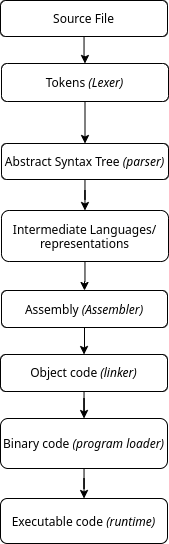
\includegraphics[width=0.25\linewidth]{CompilerFlow.png}
    \caption{Compiler Flow}%
    \label{fig:compFlow}
\end{figure}
\section{Lexical Analysis}

Lexical analysis, the job performed by the \textit{Lexer} is the first stage of compilation. It converts a source file written in a specific programming language into a string of \i{tokens}. Or alternatively, string $\implies$ list of ``lexemes''

For example, the code:


\begin{align*}
    \texttt{fold (+) [1;2] 0} &\implies \\ 
                              &\texttt{identifier open-round-bracket operator } \\ 
                              &\texttt{close-round-bracket open-square-bracket constant } \\ &\texttt{semicolon constant close-square-bracket constant}
\end{align*}


Lexemes are specified using regular expression which, in turn, are implemented using finite state automata.

For example, a simple Regular Expression capturing the \i{lexeme} of numbers:

\[
  num = \texttt{[+-]?[1-9][0-9]}^\ast
\]


Backtracking is the \i{dumb} approach to parsing regular expressions. It is also known as the brute force method as in the worst case scenario, all possibilities could be tried before the approach \i{gives up}.

Such an expression which is tricky to parse using backtracking is:

\[
  tricky = \texttt{a?a?aa}
\]


Every occurrence of the \i{optional} ($?$) doubles the number of possible routes through a parse tree of this expression. Meaning an input such as $ \texttt{aaaaa}$ would cause an evaluator to explore every possible branch of this tree before determining that it is not captured.

\subsection{Finite State Automata}

A better approach is to use Finite state automata. This approach was originally proposed by Ken Thompson. 

Using FSA our $tricky$ regex can be converted to the following Deterministic Finite State Automaton or DFA. 
\begin{center}
    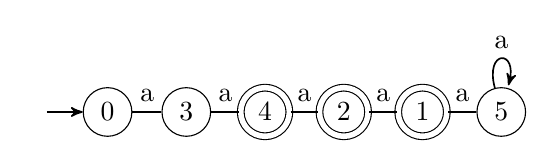
\begin{tikzpicture}
        \node [fsa-point,initial] (P1) {0};
        \node [fsa-point,right of=P1] (P2) {3};
        \node [fsa-point,accepting,right of=P2] (P3) {4};
        \node [fsa-point,accepting,right of=P3] (P4) {2};
        \node [fsa-point,accepting,right of=P4] (P5) {1};
        \node [fsa-point,right of=P5] (P6) {5};
        \draw (P1) edge node {a} (P2);
        \draw (P2) edge node {a} (P3);
        \draw (P3) edge node {a} (P4);
        \draw (P4) edge node {a} (P5);
        \draw (P5) edge node {a} (P6);
        \draw (P6) edge[loop above] node {a} (P6);
    \end{tikzpicture}
\end{center}

However, the process to create a DFA is computationally expensive. Therefore, Thompson's algorithm instead operates over Non-deterministic finite state automata. It works by keeping track of all the positions in the DFA where we could be given the string we have seen so far.

\section{Parsing}

In this stage of the process where the sequence of tokens generated by the lexer is transformed into the Abstract Syntax Tree (ASG) of the program. An ASG is a record of the grammatical structure of the program and is essential to the correct interpretation of a program. 

\subsection{Grammars}

A grammar is a set of rules. They are defined using Terminals and Non-Terminals. They are differentiated by the fact that during every application of a rule, the non-terminal occurring on the left-hand side (see below) is replaced by a sequence of terminals and non-terminals appearing on the right-hand side.

An example grammar could be:
$$
E \rightarrow N | E + E | E * E
$$

When used as a \i{production system} our rule(s) is(are) repeatedly applied to a designated starting symbol until we produce an expression comprised exclusively of terminal symbols.

For example:

\begin{align*}
    E &\rightarrow \u{E} + E &&\texttt{apply } E \rightarrow E + E \\
      &\rightarrow \u{E} * E + E &&\texttt{apply } E \rightarrow E * E \\
      &\rightarrow 42 * \u{E} + E &&\texttt{apply } E \rightarrow N \\
      &\rightarrow 42 * 35 + \u{E} && \texttt{apply } E \rightarrow N \\
      &\rightarrow 42 * 35 + 17 && \texttt{apply } E \rightarrow N
\end{align*}

We can also run this process in reverse to convert a string of terminal symbols back to the starting non-terminal $E$. 

We can however, recognise an issue with this process whereby, the set of possible operations at any given point is greater than 1. i.e. the process is \u{not} deterministic.

For example:

\begin{center}
   \begin{forest}
       [E [E [E [ 42] ]
             [*]
             [E [ 35] ]
          ]
          [+]
          [E [ 17] ] 
        ]
   \end{forest} 
\end{center}

\begin{center}
   \begin{forest}
       [E [ E [ 42] ]
          [ *]
          [ E [
                [E [ 35]]
                [+]
                [E [17]]
                ]
            ]
            ]
   \end{forest} 
\end{center}

These trees are both valid under this grammar but they are not both valid mathematically. This is because the grammar does not embed the \i{strength} of the operators.

$$
(42 * 35) + 17 \neq 42 * (35 + 17)
$$

Ambiguity and non-determinism are some of the biggest issues faced when constructing a grammar indented for use as a production system or parsing. It has been shown that the ambiguity of context-free grammars is an un-decidable problem, i.e. there is no way to construct a program that can \i{decide} whether a given grammar is ambiguous. This leads to the designing of grammars more of an \i{art} relying on the experience of the creator and the use of heuristics.

We can re-write our original grammar in a non-ambiguous way to prevent the formulation of strings that can have conflicting parse trees.


\begin{align*}
    E &\rightarrow S + S | S \\
    S &\rightarrow M * M | M \\
    M &\rightarrow ( E ) | N
\end{align*}

\begin{center}
\begin{forest}
    [E [S [M [42]]
                  [*]
                  [M [35]]
                ]
              [+]
              [S [M [17]]]
              ]
\end{forest}
\end{center}

Above you can see that our valid example can be constructed using this new grammar but below you can see that the semantically invalid tree is now also structurally invalid: 

\begin{center}
   \begin{forest}
        [ ?? [ S [ M [ 42 ] ] ]
             [ *]
             [ E [ S [ M [ 35] ] ]
                 [ + ]
                 [ S [ M [ 17 ] ] ]
                ]
            ]
   \end{forest} 
\end{center}

\subsection{Top-down parsing}
\subsubsection{Recursive Descent}
Recursive descent means we start at the \u{top} with our starting non-terminal, in this case $E$. We then apply rules until we reach a string comprised entirely of terminals, if the terminals match the string we are trying to generate then the string is valid otherwise we backtrack and apply different rules. We repeat this process until we either exhaust all possible valid combinations of rules or we match the terminals.

From the section on Lexical Analysis we know that backtracking is rarely a good solution as it has very poor worst-case complexity (exponential).

\subsubsection{LL($k$) Parsing}
There is an improved version of top-down parsing called LL(k) or left-to-right leftmost derivation with k tokens lookahead. The benefit of a \i{lookahead} is that it is able to disambiguate the application of the rule. The caveat is that the grammar has to be written in a compatible way for this system to work.

The LL(1) form of our grammar is formulated as such:

\begin{align*}
    E &\rightarrow T E' \\
    E' &\rightarrow + E | \varepsilon \\
    T &\rightarrow F T' \\
    T' &\rightarrow * T| \varepsilon \\
    F &\rightarrow N | ( E )
\end{align*}

Grammars of this type can be constructed algorithmically from an already deterministic grammar. \textbf{However,} not all grammars can be put into LL(1) form. It has been shown that it is undecidable whether given a grammar there is a fixed value of $k$ s.t. the grammar can be put into LL($k$) form.

\subsubsection{Monadic Parsing}

In order to avoid backtracking we build on the fact that we have seen that we can often replace time complexity with space complexity.

Simply speaking, in this approach we remember, inside of a data structure, the choices we have not made. i.e. in a list we store all the possible rules and evaluate all of them at the same time, discarding invalid trees until we either run out of trees or find one that is valid.
\subsection{Bottom-up parsing:}
\subsubsection{LR($k$): left-to-right rightmost derivation with $k$ tokens lookahead (LALR)}

Here we start at the \i{bottom} with our terminal string and apply rules until we reach our starting non-terminal. We again utilise $k$ lookahead to disambiguate rules as we apply them, this allows us to discount a rule earlier if we see that it doesn't reduce to a required intermediary form.

There are a few problems which can arise when using LALR parsers. 

One of these issues is known as a shift-reduce conflict. A typical example of a shift-reduce conflict is if-then-else in languages that permit both if-then and if-then-else syntactic structures. For example:

$$
\texttt{if x then if y then a else b}
$$
Is this mean to be processed as:

$$
\texttt{if x then} \{ \texttt{if y then a}\}\texttt{ else b}
$$

or 

$$
\texttt{if x then} \{\texttt{if y then a else b}\}
$$

These are usually disambiguated by the parser mechanism preferring the \i{shift} to the \i{reduce}. Essentially, always trying to construct the longest possible parses.

A more problematic type of conflict is the reduce-reduce conflict.

\begin{align*}
    \texttt{Seq} &\rightarrow \varepsilon \\
        &| \texttt{Maybe} \\
        &| \texttt{Seq }a \\
        \\
    \texttt{Maybe} &\rightarrow \varepsilon \\
          &| a
\end{align*}

Here we can derive $a$ with 2 different parse trees, either via the Seq structure or Maybe structure.

When you have one of these conflicts it is unclear which operation is going to happen and generally the execution order boils down to the order of the rules in the grammar definition.

\textbf{Note: both of these conflicts are typically unavoidable in a large grammar, mitigating them is an art rather than a science.} 

Larger parsers are generally not written by hand and are instead generated using a \textbf{Parser generator} such as \i{YACC, Bison, Parsec, etc.}

\section{Intermediate Representation}

\subsection{Abstract Syntax Trees (ASTs)}

After the parse tree is created, it needs to be processed further so that it is easier to execute/compile. 
It is easier to initially consider interpretation. We want to, given an abstract syntax tree, interpret the expression that the Abstract syntax graph represents.

For example given the input string:

$$
(1 + 2) + (3 + 4)
$$ 

We token-ise it to get:

$$
( \;\; \u{1}\;\;  \u{+}\;\;  \u{2}\;\;  )\;\;  \u{+}\;\;  (\;\;  \u{3}\;\;  \u{+}\;\;  \u{4}\;\;  )
$$

where underlined values are individual tokens.

We then construct a parse tree of this tokenised string:

\textbf{Note: the names of the terminals/non-terminals is unimportant} 

\begin{center}
    \begin{forest} for tree={grow=north, circle, draw, parent anchor=north, child anchor=south,}
    [ 
            [
                [ \u{4}]
                [ \u{+}]
                [ \u{3}]
            ]
           [[\u{+}]]
            [
                [\u{2}]
                [\u{+}]
                [\u{1}]
           ]
    ]
    \end{forest} 
\end{center}

Notice how we have removed the brackets; once the tree has been created, the brackets become implicit.
We can also push the operators onto the parent nodes to produce an equivalent but prettier Abstract syntax tree: 

\begin{center}
    \begin{forest} for tree={grow=north, circle, draw, parent anchor=north, child anchor=south}
     [+ 
        [+ 
            [\u{4}]
            [\u{3}]
        ]
        [+ 
            [\u{2}]
            [\u{1}]
        ]
     ]
    \end{forest} 
\end{center}

We can show program execution as transformations on these Abstract Syntax Trees. 
How do we know what order to apply these transformations? We use a fixed traversal method such as Depth first left-right traversal.

The application of this form of traversal on our exemplar can be seen in Figure~\ref{fig:AST1}

\begin{figure}[htpb]
    \centering
    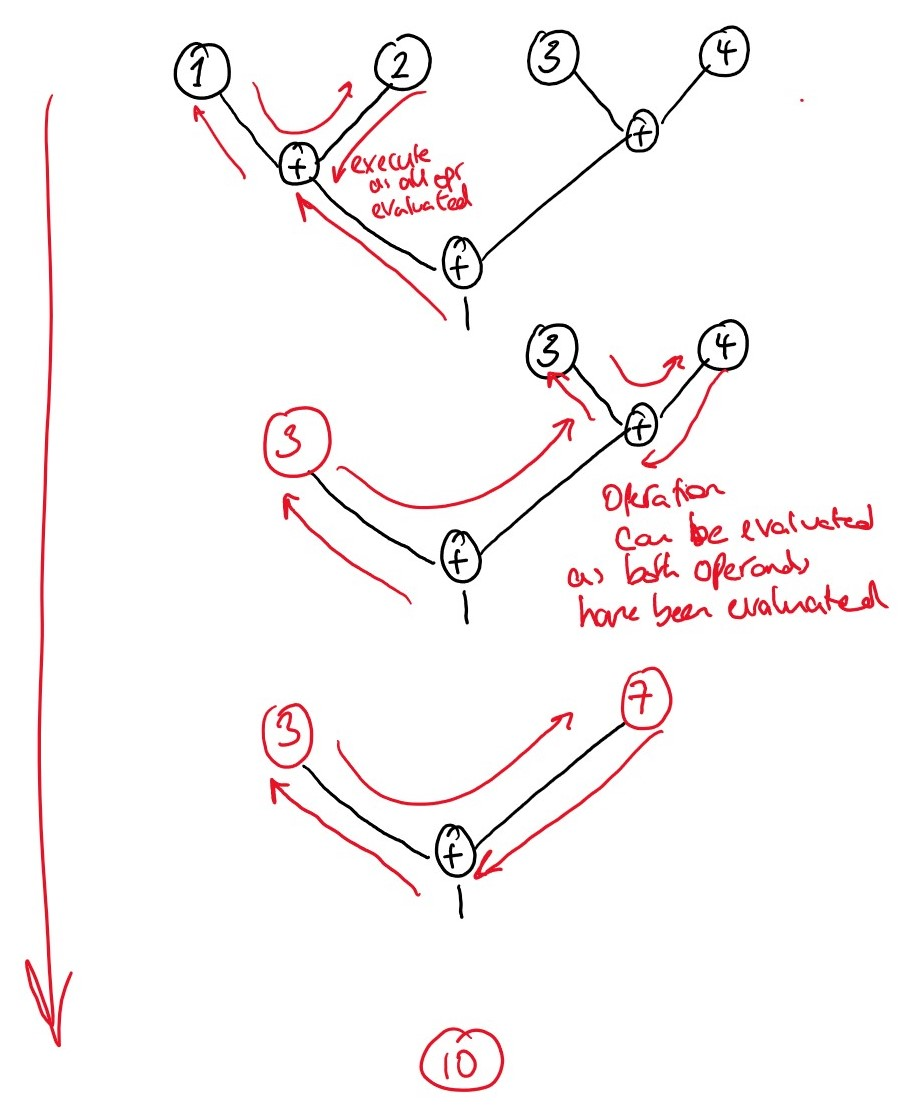
\includegraphics[width=0.6\linewidth]{c4-2.jpg}
    \caption{Depth-first L-R traversal}%
    \label{fig:AST1}
\end{figure}

ASTs do not cope well with variable names however, this is a big issue as variables are key in useful programming languages.

We will be focusing on \textbf{immutable} variables in the examples below.

$$
\texttt{let x = 1+2 in x + x}
$$

This is an example of a ternary statement, i.e. it has 3 components. It can be drawn as the following AST:

\begin{center}
    \begin{forest} for tree={grow=north, circle, draw, parent anchor=north, child anchor=south}
       [let 
           [+
            [x]
            [x]
           ]
           [+
            [2]
            [1]
           ]
           [[x]]
       ]
    \end{forest} 
\end{center}

With this representation we are left with variable names on the leaves of the tree, with no reference back to their definition. If we were to evaluate this in the same way as we did previously we produce the following tree:

\begin{center}
    \begin{forest} for tree={grow=north, circle, draw, parent anchor=north, child anchor=south}
       [let 
           [+
            [x]
            [x]
           ]
           [3]
           [[x]]
       ]
    \end{forest} 
\end{center}

When we reach the first x reference, we are forced to backtrack through the tree in order to find it's associated value. This is extremely inefficient, especially in the case where we have nested variable usage, for example in:

$$
\texttt{let x = 4+5 in let x = 3+2 in x+x}
$$

When evaluating this expression we must be careful about the scope of the variable(s) x as it has multiple definitions within the same expression. 

We must find a better solution to this problem. We do this by converting our tree into a Directed acyclic graph (DAG), turning our AST into an Abstract Syntax Graph (ASG)

\subsection{Abstract Syntax Graphs (ASGs)}

We can draw the ASG of our original $ \texttt{let}$ expression as such:

\begin{center}
   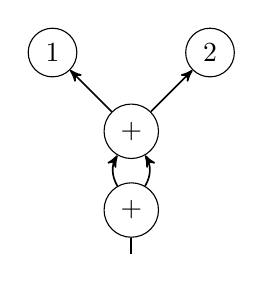
\begin{tikzpicture}
       \node[anchor=south,asg-point] (p1) {+};
       \node[asg-point,above of=p1] (p2) {+};
       \node[asg-point,left of=p2, above of=p2] (v1) {1};
       \node[asg-point, right of=p2, above of=p2] (v2) {2};
       \node[below=0.2cm of p1] (init) {};

 
       \draw (p1) edge[->,bend right] (p2);
       \draw (p1) edge[->,bend left] (p2);
       \draw (p2) edge[->] (v1);
       \draw (p2) edge[->] (v2);
       \draw (init) edge (p1);
   \end{tikzpicture} 
\end{center}

We can now apply our Depth-first left-to-right evaluation order easily and efficiently. However, rememebr we are no longer performing a tree traversal but a \textbf{graph traversal}. The evaluation of this ASG can be seen below:

\begin{figure}[htpb]
    \centering
    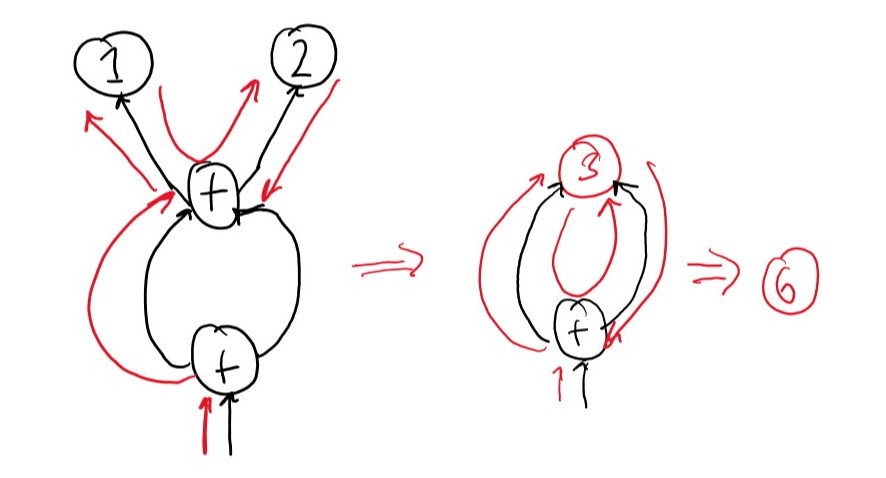
\includegraphics[width=0.5\linewidth]{c4-4.jpg}
    \caption{ASG Traversal}%
    \label{fig:ASG1}
\end{figure}

Converting from ASTs to ASGs introduces some compile-time overhead but allows for much more efficient execution of ones code. 

\subsection{Hierarchical Abstract Syntax Graphs}

Functions in the context of the $\lambda$-Calculus only have 2 operations we would need to be concerned with with respect to an abstract intermediate representation: 1) Abstraction 2) Application. How can we encode these into ASGs?

\u{Function Application}
\[
    \underbrace{x_0,\dots,x_n}_\Gamma,\underbrace{y_0,\dots,y_n}_\Delta \vdash f(m)
\]

Here we represent the identifiers of $f$ by $\Gamma$ and the identifiers of $m$ by $\Delta$.
We can consider function application as an operator. Therefore to construct an ASG of this expression, we construct the ASG of $f$ and the ASG of $m$ and combine them using an application operator, represented as @.

\begin{center}
   \begin{tikzpicture}
       \node[below=0.8cm of p1] (init) {};
       \node[circle,draw] (app) {$@$};
       \node[rectangle,minimum size=1cm,draw,above=1.5cm of app,left of=app] (f) {$f$};
       \node[rectangle,minimum size=1cm,draw,above=1.5cm of app, right of=app] (m) {$m$};
       \node[above=0.8cm of f] (abovef) {};
       \node[above=0.8cm of m] (abovem) {};
       
       \draw (abovem) -- node[strike out,draw,-,label=right:{$\Delta$}] {} (m) ;
       \draw (abovef) -- node[strike out,draw,-,label=right:{$\Gamma$}] {} (f) ;
       \draw (init) edge (app);
       \draw (app) edge[bend left] (f);
       \draw (app) edge[bend right] (m);
   \end{tikzpicture} 
\end{center}

Here the stricken through lines represent many lines ($1\ldots n$)

When we apply a function we carry out what is known as the \i{small} $\beta$ rule. It can be formulated as:

\[
    ( \lambda x.f)m \rightarrow f[m\backslash x]
\]

This is very similar to the rules we have seen in operational semantics.

\u{Function Abstraction}

\[
    x_0,\underbrace{x_1,\ldots,x_n}_\Gamma \vdash \lambda x_0.m
\]

\begin{center}
    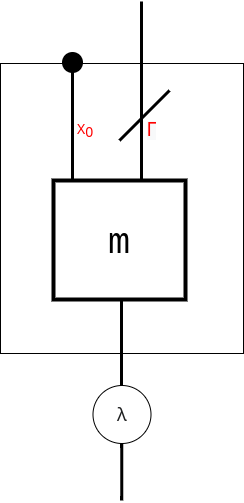
\includegraphics[width=0.3\linewidth]{ASGAbstraction.png}
\end{center}

In the above ASG you can see the representation of a $\lambda$-abstraction. The bound variable $x_0$ does not leave the scope of the abstraction (denoted by the outermost box).


\subsubsection{Examples}
\begin{enumerate}
    \item 
\[
    \lambda x.x+x+1
\]
\begin{center}
    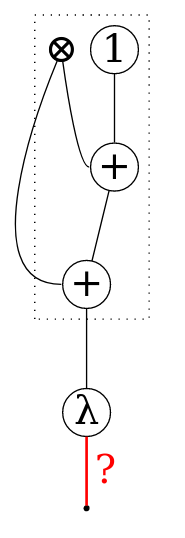
\includegraphics[height=0.5\linewidth]{ASGEx1.png} 
\end{center}
\item
\[
    \texttt{let } y = 1 \texttt{ in } \lambda x.x + x + y
\]
\begin{center}
    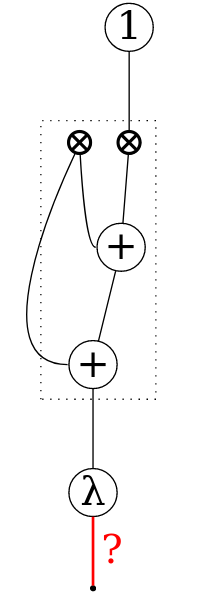
\includegraphics[height=0.5\linewidth]{ASGEx2.png} 
\end{center}

\item
\[
    \texttt{let } y = 1 \texttt{ in }
    \texttt{let } f = \lambda x.x + x + y  \texttt{ in }
    f(f(y))
\]

\begin{center}
    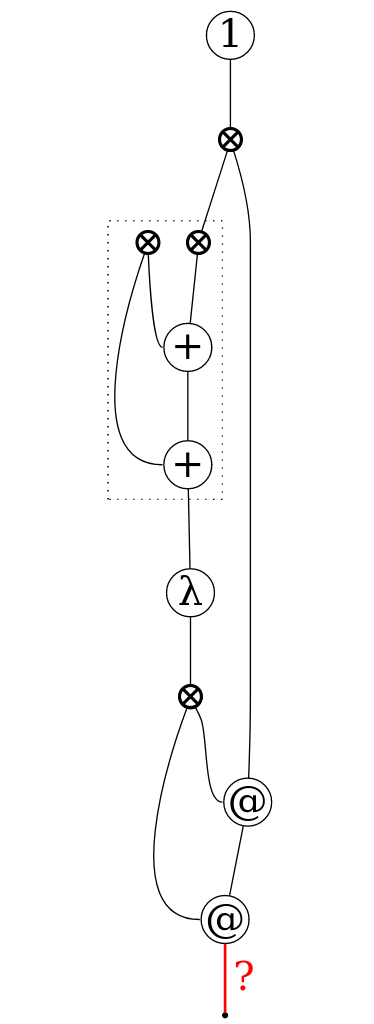
\includegraphics[height=0.6\linewidth]{ASGEx3.png} 
\end{center}

\end{enumerate}
\subsection{Note from Revision Lecture}
We must be aware of the distinction between a compiler evaluation and optimisation.

Abstractly, a evaluation is a set of abstract syntax graph transformations applied according to a schedule. For a call-by-value programming language this takes the form of a depth first search traversal of the ASG with reductions applied on the path \textit{back} up the tree towards the root.

A compiler optimisation is applying some transformations that make the code simpler and faster in an arbitrary order

A compiler optimisation is applying some transformations that make the code simpler and faster in an arbitrary order. Optimisations often have conditions that have to be met for them to be applied.
An example of a compiler optimisation is closure conversion. Closures being anonymous functions.

In a closure conversion we want to \textit{pull} inner (anonymous) functions into global scope. However, this raises an issue: what do we do with the variables of the closure which are bound in the enclosing function? We solve this using a notion of environment and transforming all functions in a uniform way.


\section{Types}

Types first appeared as an attempt to give a foundation of mathematics using the $\lambda$-Calculus via the Curry-Howard correspondence whereby a proposition corresponds to a type and a program corresponds to a proof.

Initially, the point of types in the Simply typed $\lambda$-Calculus was to ensure that a given program will always terminate. Modern usages are to prevent runtime errors in programs.

In the Curry-Howard correspondence, we can consider a value $u : T$ as a predicate $T(u)$ which states that \i{'$u$ has type $T$'}. This is what is known as a \i{type judgement}, type judgements are proved using logically formulated typing rules.

\subsection{Type Checking}

Given a program, $u$ which takes typed variables $x_0,\ldots,x_n$ we can perform a type judgement that $u$ has type $T$

\[
    x_0:T_0,\ldots,x_n:T_n \vdash u:T \;\;\; (\equiv) \;\;\; \Gamma \vdash u:T
\]

\begin{center}
   \begin{prooftree}
        \AXC{$\Gamma \vdash u : T \rightarrow T' \;\; \Gamma \vdash v:T$}
        \RL{Implication elimination}
        \UIC{$\Gamma \vdash u(v) : T'$}
   \end{prooftree} 
   \begin{prooftree}
       \AXC{$\Gamma,x :T \vdash u:T'$}
       \RL{Implication introduction}
       \UIC{$\Gamma \vdash \lambda x.u:T \rightarrow T'$}
   \end{prooftree}
\end{center}

Here it is the parallels between logical implication and functions as expressed by the Curry-Howard correspondence are clear.

We can extend this to work for other types such as Product and Sum types. For product types we have the rules:

\begin{center}
   \begin{prooftree}
       \AXC{$ \Gamma \vdash u : T_1 \times T_2$}
       \RL{Conjunction Elimination}
       \UIC{$ \Gamma\vdash proj_i(u):T_i$}
   \end{prooftree} 
   \begin{prooftree}
       \AXC{$ \Gamma \vdash u_i : T_i$}
       \RL{Conjunction Introduction}
       \UIC{$ \Gamma\vdash (u_1,u_2) : T_1 \times T_2$}
   \end{prooftree}
\end{center}

Using this pattern we can define the function types for references:

\begin{align*}
    ref_T &: T \rightarrow \texttt{ref}(T) \\
    assg_T &: \texttt{ref}(T) \rightarrow T \rightarrow ()\\
    deref_T &: \texttt{ref}(T) \rightarrow T
\end{align*}

We can go on to define increasingly complex types with this pattern, however, not all languages implement these. 
One such example is \textbf{dependant types} which are available in proof assistants such as Agda and Idris. They allow for the embedding of conditions into the type of a function, for instance the function "nth" can be defined simply as:

\begin{center}
   \begin{minted}{OCaml}
      n : Int -> (xs : 'a List) -> 'a
   \end{minted} 
\end{center}
However, this allows for runtime errors, for instance in the case where \mintinline{OCaml}{ n > length xs == true} the function would crash.

In languages with dependant types we can embed the proof that this isn't true in the type of the function: 

\begin{center}
   \begin{minted}{OCaml}
      n : Int -> (xs : 'a List) -> (n < length xs) -> 'a
   \end{minted} 
\end{center}

\subsection{Type Inference}

Type inference is the process whereby given a term, we have to decide whether it is possible to assign types to variables so that according to our typing rules our term will now typecheck.

There are various methods such as the Hindley-Milner algorithm which works by collecting a set of \i{equations} from the AST created by denoted types with variables and solving the system of equations using the principals of reduction and unification. 

The Hindley-Milner algorithm in the worst-case scenario has exponential time complexity. However it's average case is more acceptable.

\textbf{For examples of constructing the ASTs mentioned above, see the video lecture.}

\section{Assignment}

Programming languages that have operations that are not representable in the $\lambda$-Calculus have what are known as \i{side effects}. Languages that go without these features are called \i{pure}.

However, if you want to add machine dependant operations such as assignment or IO the language becomes \i{effectful} or \i{impure}

\u{Assignment}

\begin{minted}{Go}
    x := u
    x = x + 1 == x = !x + 1 //true
\end{minted}

Above you can see an example of assignment within an imperative language. The second line shows how most language add implicit de-reference when working with variable values.

More abstractly, this can be written: 

\begin{minted}{Rust}
   let x = U in V 
\end{minted}

Where U is our assigned value and V is the block in which it is in scope.
This can be represented as the following AST:

\begin{center}
   \begin{tikzpicture}
       \node[anchor=south,asg-point] (eq) {:=};
       \node[above left of=eq] (lhs) {variable};
       \node[above right of=eq] (rhs) {value};
       \node[below=0.2cm of eq] (init) {};

 
       \draw (eq) edge[bend right] (rhs) ;
       \draw (eq) edge[bend left] (lhs) ;
       \draw (init) edge (p1);
   \end{tikzpicture} 
\end{center}

\begin{center}
   \begin{tikzpicture}
       \node[anchor=south,asg-point] (eq) {!};
       \node[above of=eq] (lhs) {variable};
       \node[below=0.2cm of eq] (init) {};

       \draw (eq) edge (lhs) ;
       \draw (init) edge (p1);
   \end{tikzpicture} 
\end{center}

\begin{center}
    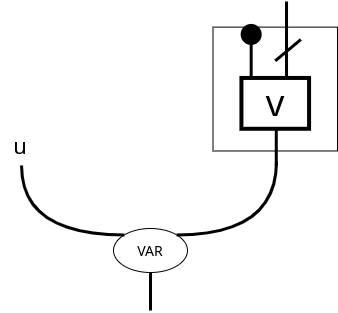
\includegraphics[width=0.2\linewidth]{VarAST.png}
  \end{center}

  Above you can see that we represent a variable, $v$ as a \textit{thunk}. This is an alternative use for thunks, we previously used them when constructing functions, notice in this case we omit the bottom $\lambda$ node.

  \u{Example}

\[
  \texttt{var x = 0 in x := !x + 1}
\]


\begin{center}
   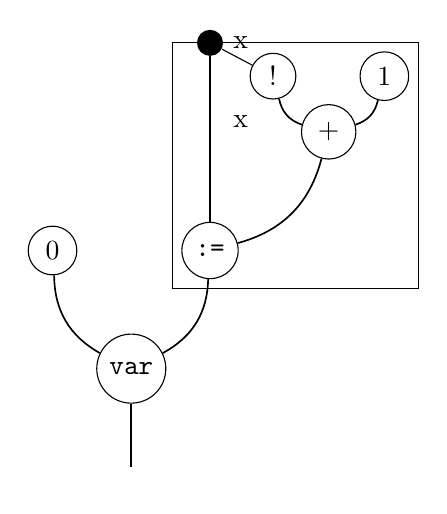
\begin{tikzpicture}

       \node[circle,draw] (var) {$\texttt{var}$};
       \node[below=0.8cm of var] (init) {};
       \node[circle,draw,above=1.5cm of var,left of=var] (zero) {$0$};

       % Thunk
       \node[circle,draw,above=1.5cm of var, right of=var] (assign) {$\texttt{:=}$};
       \node[circle,draw,above right=of assign] (plus) {$+$};
       \node[circle,draw,above left of=plus] (bang) {!};
       \node[circle,draw,above right of=plus] (v1)  {$1$};
       \node[circle,fill,above=2.1cm of assign] (border) {};
       \node[draw,fit=(assign) (plus) (bang) (v1)] {};

       \draw (var) edge[bend left] (zero);
       \draw (var) edge[bend right] (assign);

       \draw (assign) edge[bend right] (plus);
       \draw[bend left] (assign) -- (border) node[below of=border,right= 0.003mm of border] {x};

       \draw (plus) edge[bend left] (bang);
       \draw (plus) edge[bend right] (v1);

       \draw[bend left] (bang) -- (border) node[below= 0.01mm of border,right= 0.003mm of border] {x};

       \draw (init) edge (var) {};

   \end{tikzpicture}
 \end{center}

 Parsing this depth-first left-to-right we find values on both sides of our $\texttt{var} $ operation. Informally, our rewrite operation will be:

 \begin{itemize}
   \item allocate/ create variable
   \item initialise to 0
   \item bind to x
 \end{itemize}

 This produces the following ASG:

 \begin{center}
   \begin{tikzpicture}

       \node[below=0.8cm of assign] (init) {};
       \node[circle,draw,above=1.5cm of var, right of=var] (assign) {$\texttt{:=}$};
       \node[circle,draw,above right=of assign] (plus) {$+$};
       \node[circle,draw,above left of=plus] (bang) {!};
       \node[circle,draw,above right of=plus] (v1)  {$1$};

       \node[circle,draw,above of=bang] (xvar) {};
       \node[circle,draw,left=14mm of assign] (zero) {$0$};

       \draw (assign) edge[bend right] (plus);
       \draw[bend left] (assign) edge[bend left] (xvar) ;

       \draw (plus) edge[bend left] (bang);
       \draw (plus) edge[bend right] (v1);

       \draw[bend left] (bang) edge[bend right] (xvar);
       \draw (xvar) edge[bend right] (zero);
   \end{tikzpicture}
 \end{center}

\section{Code Generation}

\begin{displayquote}
   'Abstract machines give you the cake.'\\
   'Compilers give you the recipe.'\\
   ---Dan Ghica
\end{displayquote}

Only touched on briefly due to complexity. Essentially, code generation is the final process of compilation. If Abstract machines execute the program, Compilers (via code generation) say what to do. 

\section{Tips for the Exam}
\begin{enumerate}
    \item Very similar to the summative assignment.
    \item Use \textit{SPARTAN}
\end{enumerate}


\end{document}

%%% Local Variables:
%%% TeX-command-extra-options: "-shell-escape"
%%% End:
